\chapter{Problem Statement, Goals, and Research Methodology}\label{chap:methodology}

The goal of this thesis is to advance the state-of-the-art in neurosymbolic AI by introducing a design method. This chapter presents the limitations detected in the state-of-the-art that motivate the research conducted in this thesis (Section \ref{3_sec:limitations}). Section \ref{3_sec:problem_statement} depicts the research problem addressed, outlining the hypotheses, goals, contributions, assumptions, and restrictions. The research methodology followed in this thesis is presented in Section \ref{3_sec:research_methodology}.

\section{State-of-the-art Limitations}\label{3_sec:limitations}
After analyzing the state-of-the-art, the following limitations were identified, which motivate the research presented in this thesis:
\begin{itemize}
    \item \textbf{Predefined roles for symbolic and subsymbolic models.} \cite{besold_neural-symbolic_2017} introduce a set of principles for neurosymbolic integration. One of the key aspects of this work is the distinction between representation and reasoning in neurosymbolic systems. This work denotes that symbolic models are used for representation, while subsymbolic models are used for reasoning. This statement is further validated by the work of \cite{garcez_neural-symbolic_2019}. The use of symbolic models as reasoning paradigms is therefore dismissed and not explored.
    
    \item \textbf{Integrations are mostly limited to rule-based systems and neural networks.} The AI spectrum, as outlined in Section \ref{sec:the_ai_spectrum}, comprises a wide variety of paradigms. In neurosymbolic systems, however, only rule-based systems and neural networks are featured, leaving a wide range of both symbolic and subsymbolic approaches unexplored. 
    
    \item \textbf{Limitations of neurosymbolic integration are not explored.} Most works in neurosymbolic design focus on the benefits or positive aspects derived from the integration of symbolic and subsymbolic models. The specific limitations that motivate certain neurosymbolic integrations are not outlined. This gives a biased perspective on the subject, as only presents the positive aspects.
    
    \item \textbf{Absence of guidelines on when and how neurosymbolic integration should be performed.} Another remarkable limitation is the absence of guidelines and case scenarios where neurosymbolic integration should be performed. Design proposals focus only on the representation and reasoning aspects of the integration, but do not consider potential issues such as computational costs, performance restrictions, or contextual elements. 
\end{itemize}


\section{Problem Statement} \label{3_sec:problem_statement}
This thesis presents a design method for hybrid learning models, focusing on the integration of knowledge-based systems (KBS) and deep learning (DL) models. The proposed design method not only comprises theoretical aspects on the integration, but functional and technical aspects that are unaddressed by previous approaches.  Moreover, it enables the integration of a wide variety of KBS and DL models in addition to the baseline integration of rule-based systems and neural networks.  

Several neurosymbolic system categorizations were outlined in Section \ref{2_sec:subsec:categorization}, each focusing on a different aspect. This thesis proposes a categorization based on the integration mechanism: introduction (or insertion), and extraction. Insertion approaches combine KBS and DL models under a unified framework to perform a task. In extraction, one of the models is either mined or used to mine knowledge from the other. 

\begin{figure}[t]
    \centering
    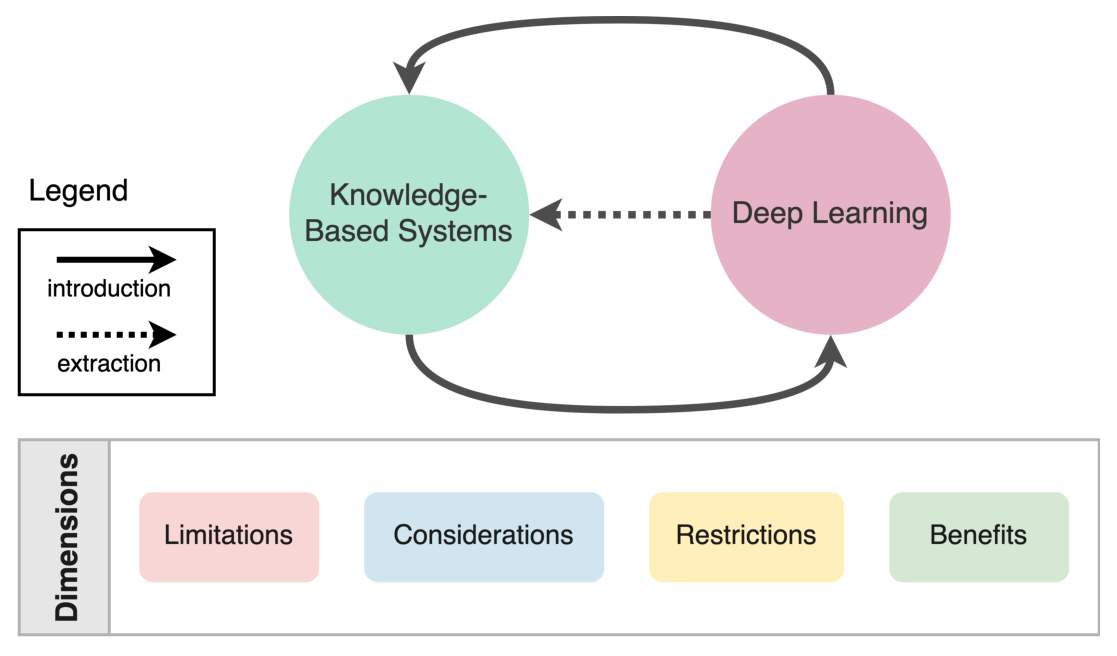
\includegraphics[width=.9\linewidth]{3_objectives/figures/overview_method.eps}
    \caption{Overview on the integration approaches and method design parameters proposed in this thesis.}
    \label{fig:thesis_overview}
\end{figure}

Figure \ref{fig:thesis_overview} showcases the three possible interactions between KBS and DL according to the aforementioned perspective: KBS insertion into DL models, DL introduction into KBS, and KBS extraction from DL models. While the introduction is bidirectional, the extraction is only directed from DL to KBS. According to the provided definition for extraction, DL extraction from KBS is unfeasible, and it is therefore not considered in this thesis. 

This thesis presents a design method for the representation of each of the three possible interactions between KBS and DL. Besides studying the potential benefits and the existing limitations of each model that motivate the integration, this method also contemplates previous requirements, as well as a set of criteria that must be met for the integration to be successful. The proposed design method comprises four dimensions, which are defined in a sequential order:
\begin{itemize}
    \item \textbf{Limitations.} Integration is motivated by the existence of limitations in one of the paradigms that could be resolved with the inclusion of a model from the opposite side of the spectrum. Limitations must be clearly identified before the integration. Model selection is based on the detected limitations and the goal of the system. This dimension only alludes to the model features.
    
    \item \textbf{Considerations.} Limitations must be framed into context. This dimension relates to the practical and contextual aspects of the integration. Infrastructural, user-related, and data aspects are depicted in this dimension.
    
    \item \textbf{Restrictions.} Integration carries an effort and serves a purpose. The effort made must not only be reflected in the results, but must also comply with a series of restrictions. Restrictions ensure that the integration not only is successful, but also that it is coherent and that the neurosymbolic system is justified for the given task and context.
    
    \item \textbf{Benefits.} A successful neurosymbolic integration entails a series of benefits. These benefits must be addressed in the context of the previously described limitations, and must be a direct result of the integration. This dimension should highlight the attainment of features that could not have been obtained otherwise.
\end{itemize}

\subsection{Research Hypotheses}
Once the research problem has been described, the following research hypotheses are formulated:
\begin{enumerate} [start=1,label={\bfseries H\arabic*:}]
    \item A design method for the integration of knowledge-based systems and deep learning models can be proposed to accurately describe most integration instances. 
    \item Knowledge-based systems and deep learning models are not antagonistic, but complementary, and their integration can facilitate the resolution of several research tasks.
\end{enumerate}

\subsection{Goals}
The main goal of this thesis is to propose a general design method for the integration of knowledge-based systems and deep learning models.  The proposed design method not only focuses on the motivation and benefits, but tackles the technical and contextual aspects that are needed to define a successful integration. For this purpose, three objectives are defined:
\begin{enumerate}[start=1,label={\bfseries O\arabic*:}]
    \item Define a set of general parameters per dimension for the integration of knowledge-based systems and deep learning models.
    \item Instantiate the proposed design method across different models and use scenarios.
    \item Assess the compliance of each implementation with respect to the general design parameters. 
\end{enumerate}

\subsection{Contributions}
According to the proposed goals, the contributions can be grouped into two categories: interaction design methods and resources.
Regarding the interaction design methods, the contributions are as follows:
\begin{enumerate}[start=1,label={\bfseries C\arabic*:}]
    \item A design method for the insertion of knowledge-based systems into deep learning models.
    \item A design method for the insertion of deep learning models into knowledge-based systems.
    \item A design method for knowledge-based system extraction from deep learning models.
\end{enumerate}
The design models depicted in contributions \textbf{C1, C2} and \textbf{C3} are instantiated on different use cases, generating the following resource contributions:
\begin{enumerate}[start=4,label={\bfseries C\arabic*:}]
    \item A semantic-based initialization method for knowledge graph embedding models.
    \item A modular case-based reasoning framework powered by deep learning models for medical document generation.
    \item A multi-agent system architecture for the extraction of behavioral patterns from black-box hyperpersonalization systems.
    \item GEnI (Generating Explanations and Insights for knowedge graph embedding predictions).
\end{enumerate}


\begin{sidewaysfigure}
  \centering
  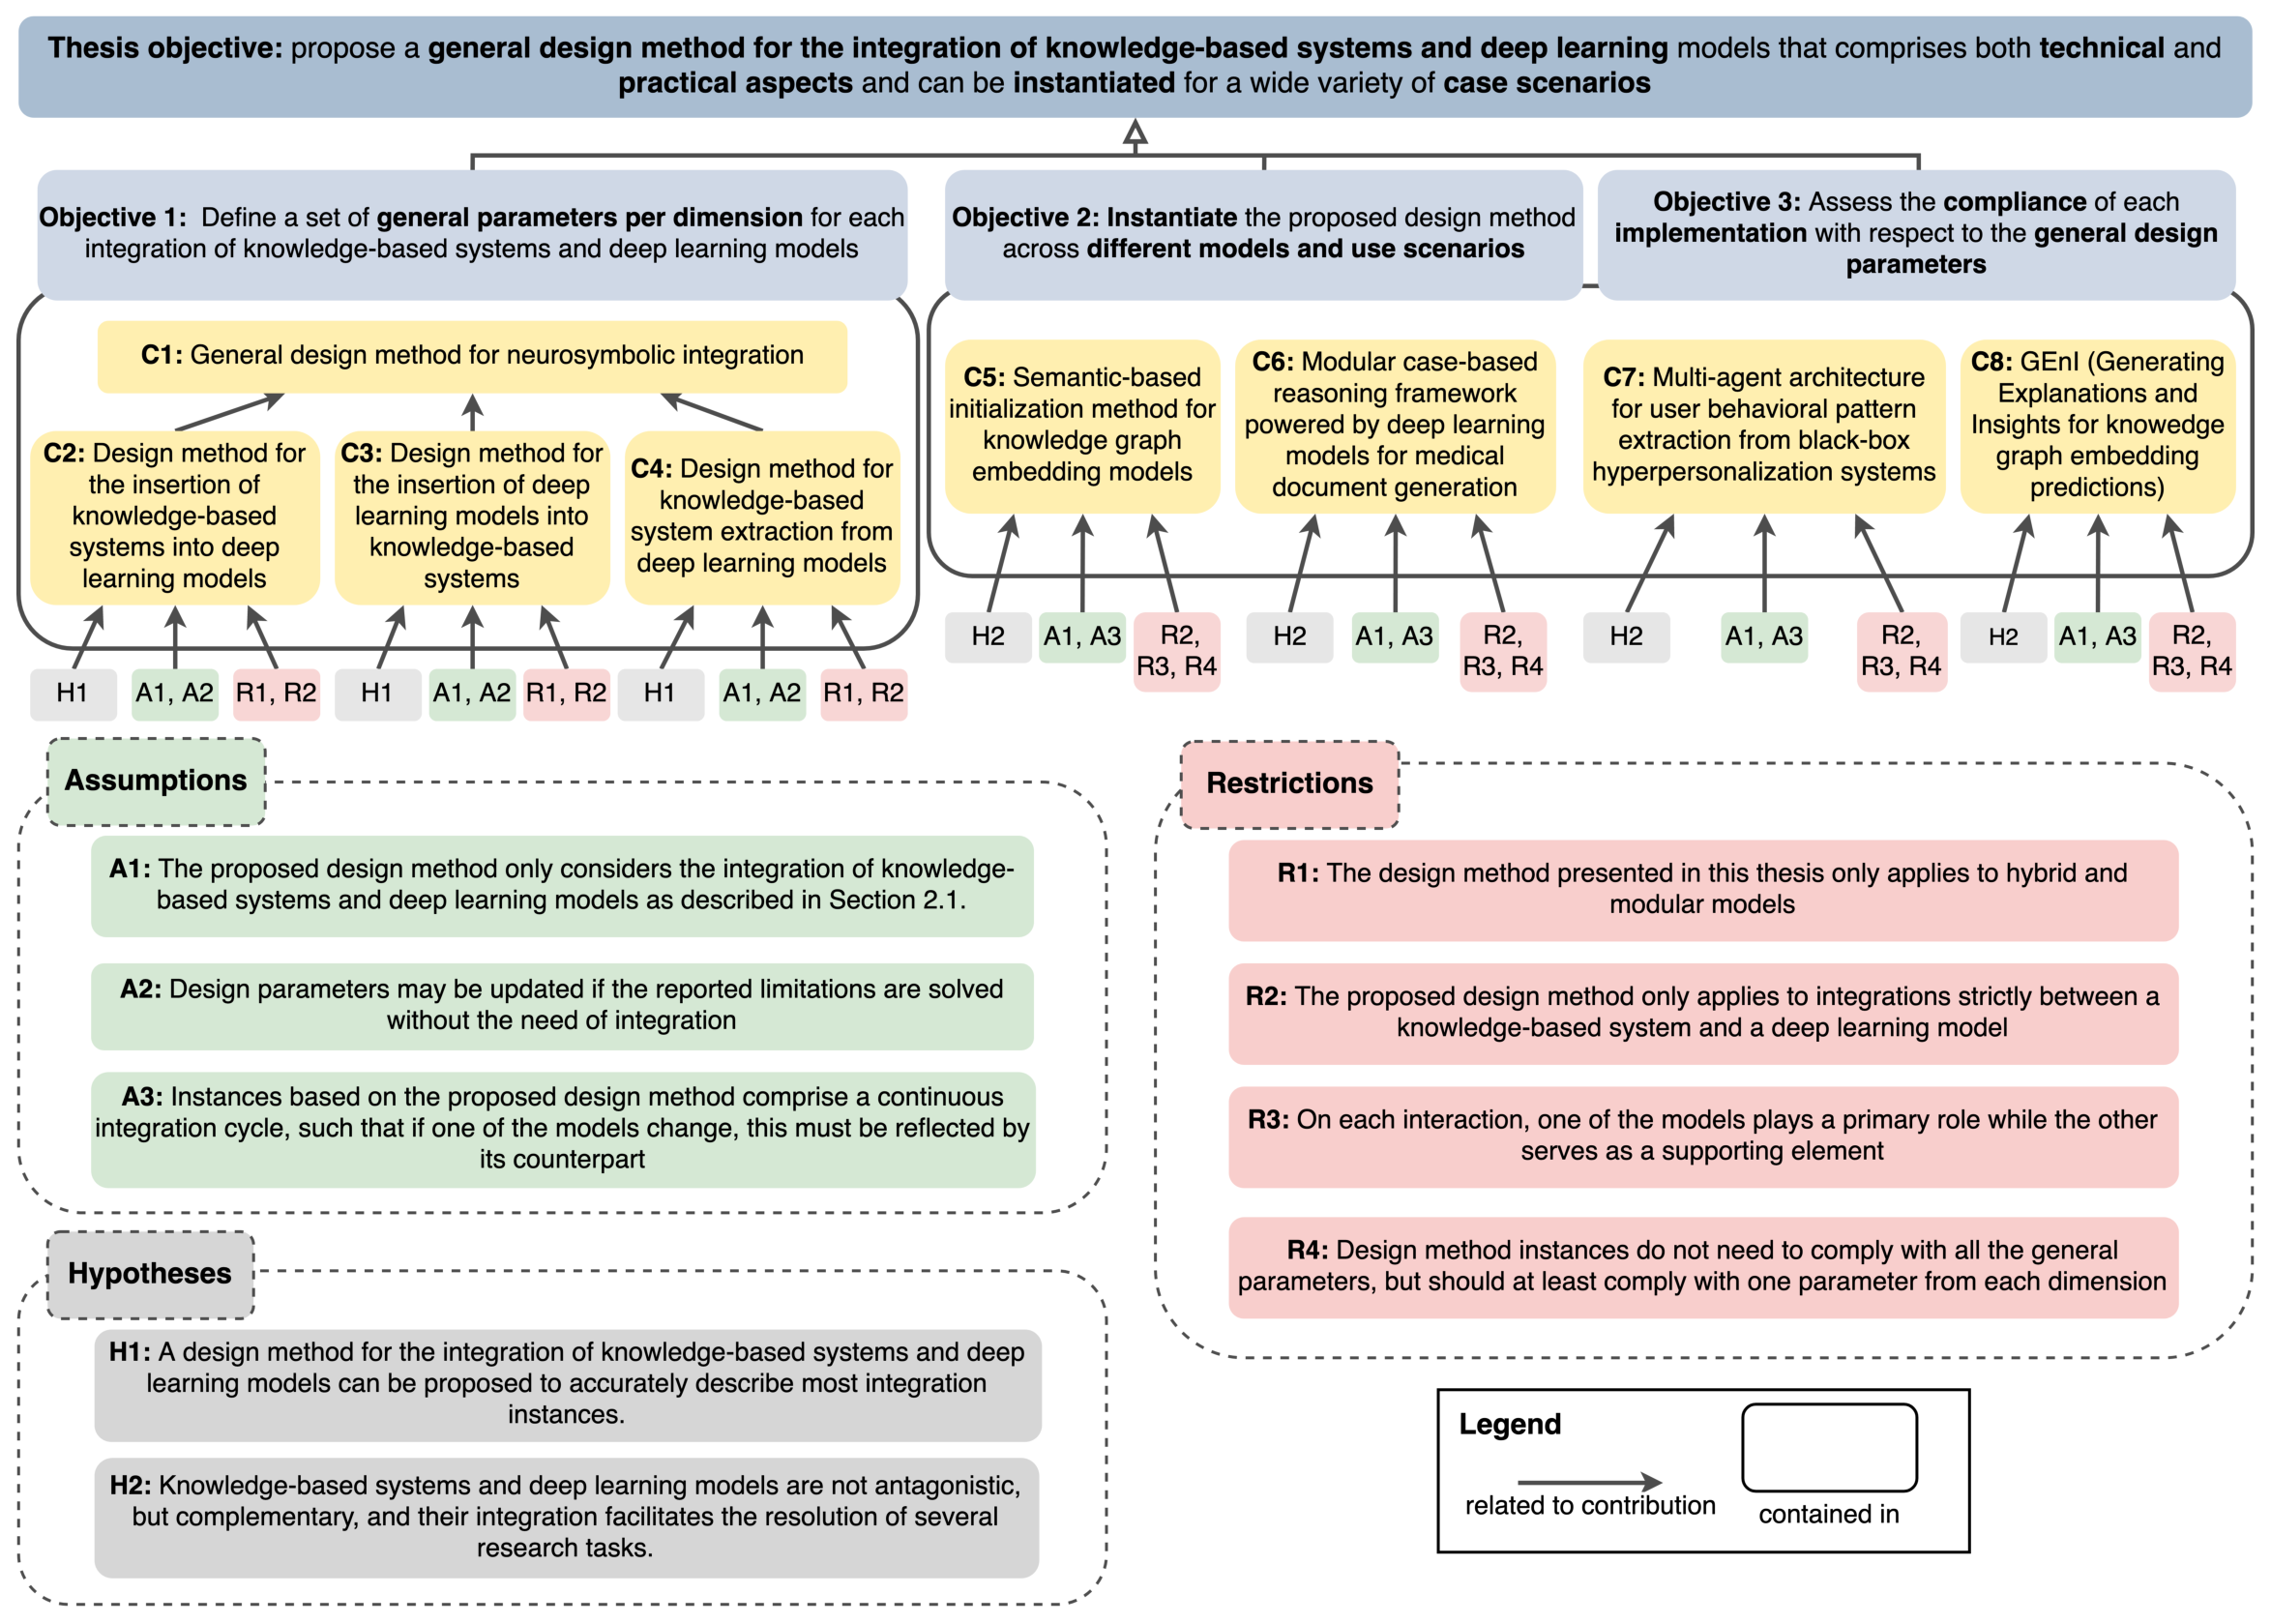
\includegraphics[width=\linewidth]{3_objectives/figures/methodology_general.eps}
  \caption{Correspondences between objectives, contributions, assumptions, hypotheses, and restrictions.}
  \label{fig:methodology_general}
\end{sidewaysfigure}

\subsection{Assumptions}
The work in this thesis is developed under the following assumptions:
\begin{enumerate}[start=1,label={\bfseries A\arabic*:}]
    \item The proposed design method only considers the integration of knowledge-based systems and deep learning as described in Section \ref{sec:the_ai_spectrum}.
    \item Design parameters for each interaction may be updated if any of the reported limitations are solved without the need of integration.
    \item Instances based on the proposed design method comprise a continuous integration cycle, such that if one of the models changes, this must be reflected by its counterpart.
\end{enumerate}
\subsection{Restrictions}
The following restrictions limit the contributions of this thesis and may be used to lead future research:
\begin{enumerate}[start=1,label={\bfseries R\arabic*:}]
    \item The design method presented in this thesis applies to hybrid models \citep{hilario_overview_nodate} and modular models \citep{mcgarry_hybrid_1999}.
    \item The proposed design method applies to integrations between a knowledge-based system and a deep learning model. 
    \item On each interaction, one of the models plays a primary role while the other acts as a supporting (secondary) element. Note: In KBS extraction from DL models, the primary model is the one that performs the extraction, while the secondary is the one where the knowledge is extracted from.
    \item Design method instances do not need to comply with all the general parameters, but should at least comply with one parameter from each dimension. 
\end{enumerate}

Figure \ref{fig:methodology_general} depicts the hypotheses, goals, contributions, assumptions, and restrictions, highlighting the relations between them. 

\section{Research Methodology}\label{3_sec:research_methodology}

\begin{figure}
    \centering
    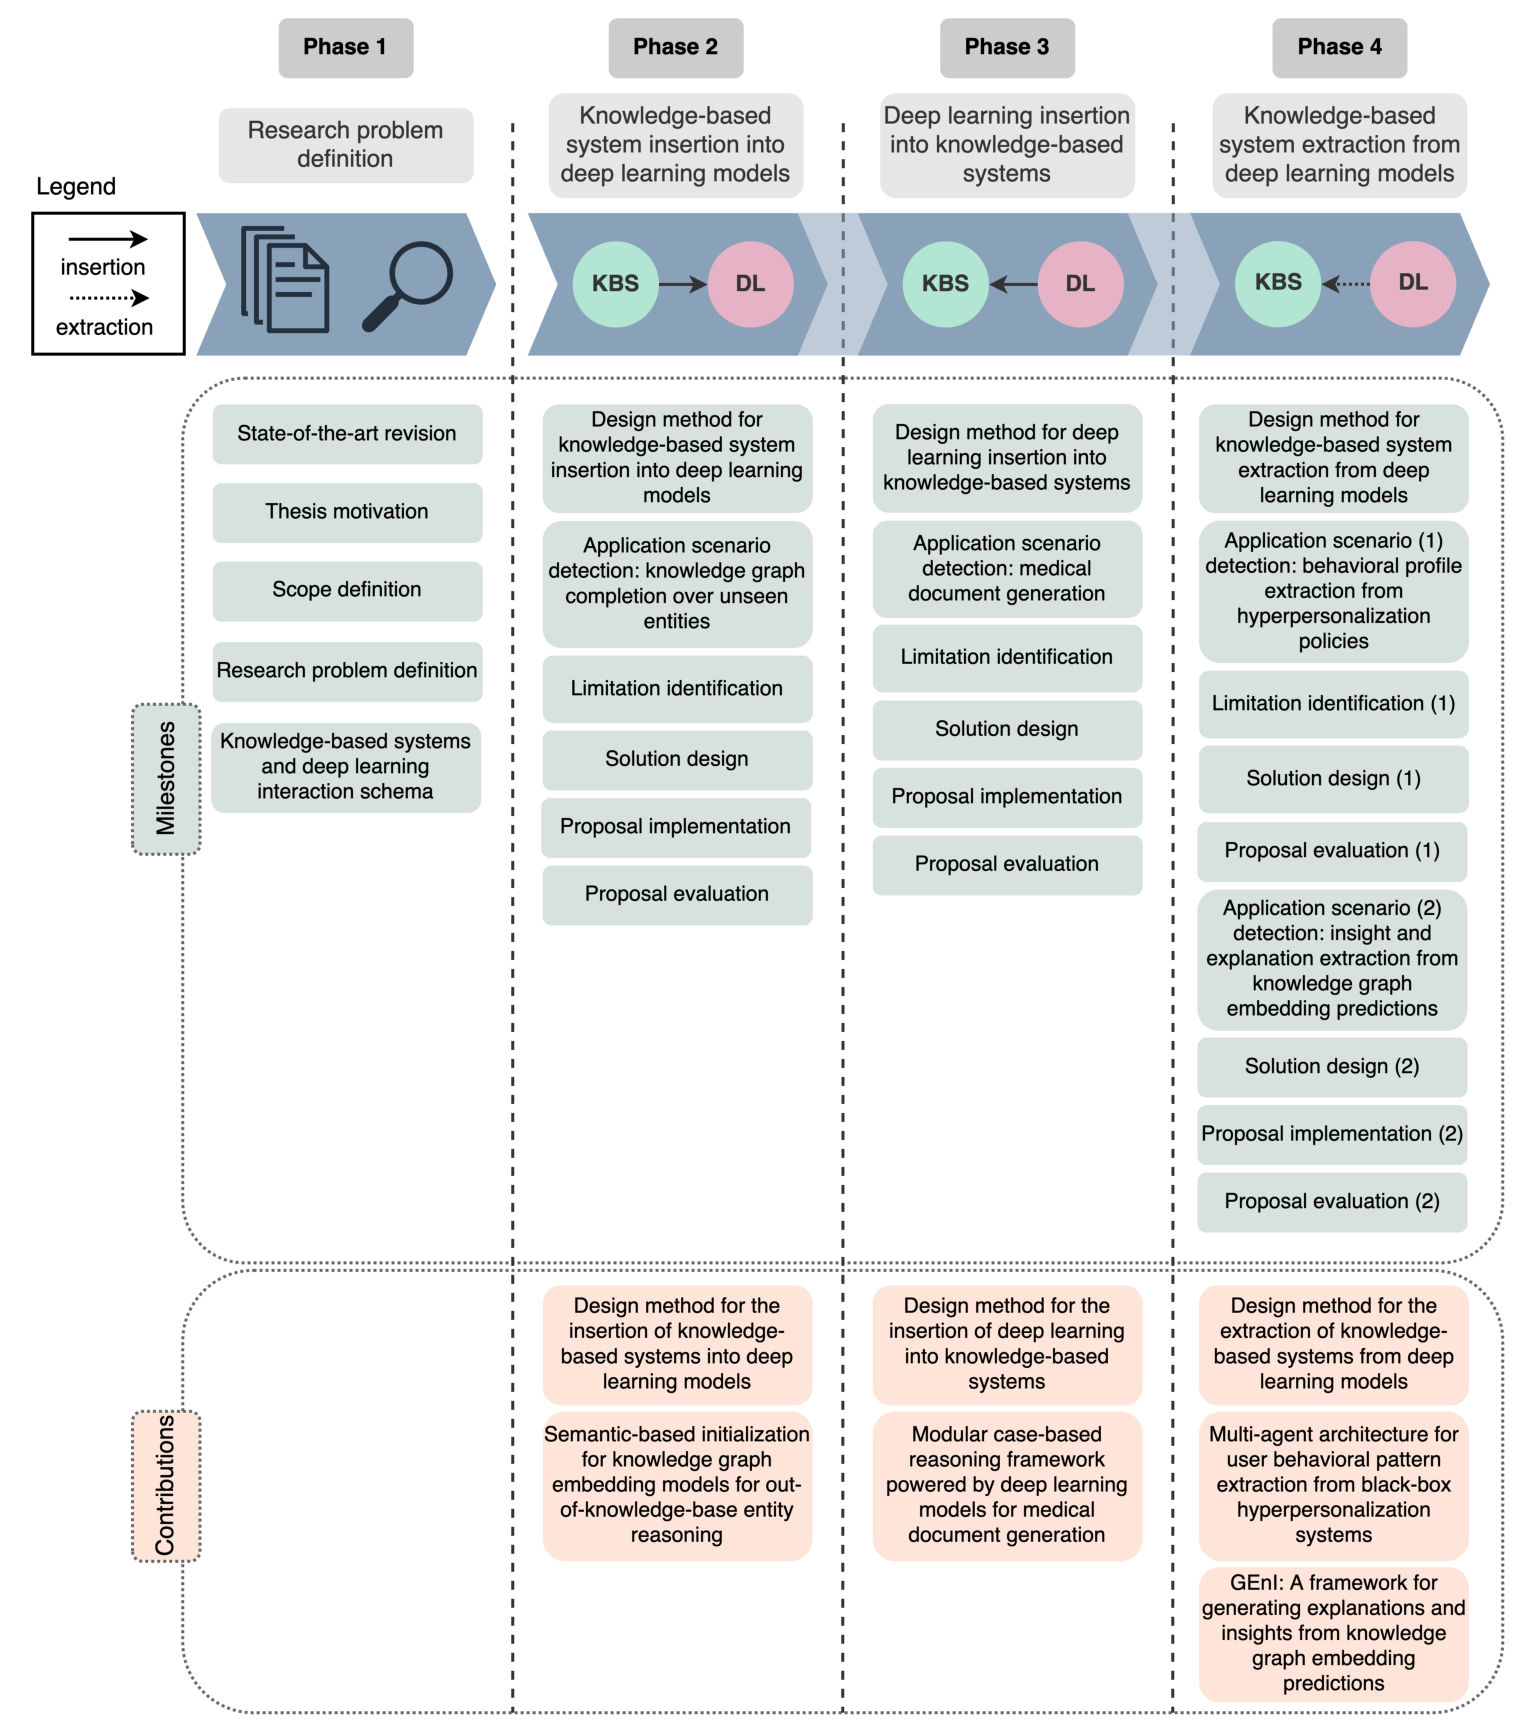
\includegraphics[width=\linewidth]{3_objectives/figures/research_methodology.eps}
    \caption{Iterative research process followed in this thesis.}
    \label{fig:research_method}
\end{figure}

The research methodology employed in this thesis follows an incremental strategy. Figure \ref{fig:research_method} outlines the general research procedure, showcasing the research milestones and contributions generated. The procedure is divided into four phases. The first phase corresponds to the study of the state-of-the-art and the definition of the research problem. Phases two, three, and four correspond to each of the interactions between KBS and DL modeled in this thesis. Phases from two to four are not executed in a strictly sequential order, as there exists a slight overlap between the end of each phase and the beginning of the following. The tasks, milestones, and contributions achieved on each phase are described as follows:
  
\begin{itemize}
    \item \textbf{Phase 1. Research problem definition.} This phase corresponds to the initial stages of the thesis. First, a state-of-the-art revision regarding neurosymbolic integration in the context of ambient intelligence was conducted. This revision helped outline the main limitations and motivations for neurosymbolic integration, which found the motivation of this thesis. Moreover, it evidenced that despite the heterogeneity between the featured symbolic approaches, most of the subsymbolic approaches were based on deep learning. Therefore, the scope of this thesis narrowed down the integration to two subcategories of symbolic and subsymbolic AI: knowledge-based systems and deep learning models. 
    
    The revision was then extended to existing neurosymbolic design proposals, from which the limitations exposed in Section \ref{3_sec:limitations} were drawn. The research problem addressed in this thesis was then formulated based on the detected limitations, motivation, and scope: defining a design method for knowledge-based systems and deep learning models. Three potential interactions between the two approaches were detected: KBS insertion into DL models, DL insertion into KBS, KBS extraction from DL models. A specific design model for each interaction is required. Moreover, these designs must be instantiated in appropriate use-case scenarios to assess the applicability of the proposal.
    
    \item \textbf{Phase 2. Knowledge-based system insertion into deep learning models.} After defining the potential interactions between KBS and DL models, the first of the interactions is studied: the insertion of KBS into DL models. The initial step of this phase defines the appropriate design parameters to perform the introduction. The validity of this design is then assessed through its implementation on a use case. Knowledge graph completion (KGC) is selected as the case scenario, as it offers a challenging and conductive environment for the application of neurosymbolic models. First, the limitations existing within knowledge graph embedding (KGE) models, the main paradigm of KGC, are identified. KGE models act as the primary DL model in the integration, while ontologies are selected as the KBS counterpart. This solution is then materialized into a semantic-based initialization proposal, being one of the contributions of this thesis. The proposed instantiation is then evaluated not only on its technical effectiveness, but on its compliance with the general design method.
    
    \item \textbf{Phase 3. Deep learning insertion into knowledge-based systems.} The second phase tackles the second of the interactions: the insertion of DL models into a KBS. Similar to the previous phase, the first milestone of this phase is the definition of the interaction general design method, where KBS and DL models are treated as a whole. As outlined in the limitations (Section \ref{3_sec:limitations}), one of the main setbacks of the studied neurosymbolic designs is the assignment of representation and reasoning roles to symbolic and subsymbolic models, respectively. Moreover, rule-based systems are the predominant symbolic paradigm, thus discarding potential alternative paradigms. In the proposed integration, the KBS also acts as a reasoning model. 
    
    Knowledge-based systems are particularly predominant in the medical domain, where user input integration and inference interpretability are essential. In this context, medical document generation provides an interesting setting for method instantiation, where the KBS plays the primary role and is enhanced by DL.  A case-based reasoning model is used in this context to play the KBS role. The limitations of this model are first addressed, devising an integrated solution that is subsequently implemented and evaluated. The compliance of the proposed implementation with respect to the design method is also assessed. 
    
    \item \textbf{Phase 4. Knowledge-based system extraction from deep learning models.} The final phase of the research comprises KBS extraction from DL models. As in phases two and three, the first step comprises the definition of the design method parameters. This final phase provides a case scenario with a higher complexity than the previous two. Explainable AI is the main open research problem in this area, whose goal is extracting symbolic knowledge from deep learning models. In this context, the DL model acts as the secondary model, while the KBS (or an intermediate model required for the extraction) acts as the primary. Under this subject, two application scenarios are considered, showcasing the versatility and adaptability of the proposed design method. 
    
    The first scenario focuses on \textit{black-box hyperpersonalization online systems}, deep learning models that generate personalized content based on passively user-retrieved data. The DL model in this context is targeted to human users, and therefore a paradigm capable of accurately simulating them is required to extract behavioral patterns. After identifying the problem limitations, a solution is designed based on a multi-agent system. The solution is then presented in the context of a case study to exemplify the behavior and adequacy of the system. Finally, the proposed integration solution is evaluated with respect to the parameters of the general design to ensure its compliance.
    
    The second scenario refocuses on KGC, extending the research from Phase 2. While the research conducted in this area focused on enhancing the performance of KGE models, the research conducted in this phase aims to explain the inference process followed by these models to generate predictions. The limitations of KGE models are then addressed under the extraction perspective. A rule-supported framework is devised to deal with these limitations. The proposed framework is implemented and evaluated both in the context of the case scenario and with respect to the general design parameters. 
\end{itemize}